\documentclass[12pt,a4paper,oneside,article]{memoir}



% LAYOUT
\usepackage{changepage}
\setulmarginsandblock{0.7\uppermargin}{0.8\lowermargin}{*}

% MATHS
\usepackage{amsmath,amsfonts,amssymb,amsbsy,commath,mathtools,calc}
\mathtoolsset{showonlyrefs,showmanualtags}

\usepackage{subfig}
% FONTS & LANGUAGE
\usepackage[usenames,dvipsnames]{color}
\definecolor{light-gray}{gray}{0.8}
\usepackage{fontspec,xltxtra,polyglossia}
\setmainlanguage{english}
\usepackage[normalem]{ulem} % have underlinings work
%\defaultfontfeatures{Ligatures=TeX}
\defaultfontfeatures{Mapping=tex-text}

\setmainfont[Ligatures={Common}, Numbers={OldStyle}]{Linux Libertine O}
%\setmainfont{Droid Sans}
%\setsansfont[Scale=MatchLowercase]{Inconsolata}
\setmonofont[Scale=0.8]{DejaVu Sans Mono}

% PDF SETUP
\usepackage[unicode,bookmarks, colorlinks, breaklinks,
pdftitle={T-61.3040: Ex 9},
pdfauthor={Ville Väänänen},
pdfproducer={xetex}
]{hyperref}
\hypersetup{linkcolor=black,citecolor=black,filecolor=black,urlcolor=MidnightBlue} 

\usepackage[backref=true, backend=biber]{biblatex}
\addbibresource{../bibliography.bib}

% TABLES
\usepackage{booktabs}
\usepackage{topcapt} 
\usepackage{rccol}
\usepackage{tabularx} % requires array
\newcommand{\otoprule}{\midrule[\heavyrulewidth]}
\newcolumntype{d}[2]{R[.][.]{#1}{#2}}

\usepackage{titlesec}
\usepackage{todonotes}

%%%%%%%% OMAT KOMENNOT %%%%%%%%%%%%

\usepackage{mymath}
\usepackage{mylayout}


% PARAGRAPHS
%\usepackage{parskip}

% kuvat

\usepackage{listings}
\lstset{ %
	language=R,                % choose the language of the code
	basicstyle=\footnotesize\ttfamily,% the size of the fonts that are used for the code 
	numbers=none,                   % where to put the line-numbers
	numberstyle=\footnotesize\ttfamily,      % the size of the fonts that are usedfor the line-numbers 
	stepnumber=5,                   % the step between two line-numbers. If it's 1 each line 
	aboveskip=2\medskipamount,
	belowskip=2\medskipamount,                                % will be numbered
	numbersep=-5pt,                  % how far the line-numbers are from the code
	backgroundcolor=\color{white},  % choose the background color. You must add \usepackage{color}
	showspaces=false,               % show spaces adding particular underscores
	showstringspaces=false,         % underline spaces within strings
	showtabs=false,                 % show tabs within strings adding particular underscores
	frame=l,
	framesep=0pt,
	framexleftmargin=2mm,
	rulecolor=\color{light-gray},	                % adds a frame around the code
	tabsize=2,	                % sets default tabsize to 2 spaces
	caption=,
	captionpos=t,                   % sets the caption-position to bottom
	breaklines=true,                % sets automatic line breaking
	breakatwhitespace=false,        % sets if automatic breaks should only happen at whitespace
	emptylines=*1,
	keywordstyle=\color[rgb]{0,0,1},          % keywords in blue
    commentstyle=\color[gray]{.5}\itshape,               % comments
    stringstyle=\color[rgb]{.627,.126,.941},   % strings in purple
	%title=\lstname,                 % show the filename of files included with
	                                % also try caption instead of title
	escapeinside={\%*}{*)},         % if you want to add a comment within your code
            % if you want to add more keywords to the set
}
 
\newcommand{\course}{S-114.4202}
\newcommand{\coursename}{Special Course in Computational Engineering II}
\newcommand{\duedate}{\today}
\newcommand{\studentid}{63527M}
\renewcommand{\title}{Lansing woods}
\author{Ville Väänänen}

\setsecnumdepth{subsubsection}
\counterwithout{section}{chapter}
\pagestyle{plain}
\makeevenhead{headings}{\course}{\Large\title}{\author / \studentid}
\makeoddhead{headings}{\course}{\Large\title}{\author / \studentid}
\makeheadrule{headings}{\textwidth}{\normalrulethickness}
\makeheadposition{headings}{flushleft}{flushleft}{flushleft}{flushleft}
\checkandfixthelayout
%\renewcommand{\thesubsubsection}{\thesubsection{\large\scshape\alph{subsubsection}}}
\newfontfamily\subsubsectionfont[Letters=SmallCaps]{Linux Libertine O}
%\titleformat{\subsection}{\large\scshape}{\alph{subsection} )}{10pt}{}
%\titleformat{\section}{\Huge}{Round \thesection}{10pt}{}
%\titleformat{\section}{\Large}{Exercise \thesection}{10pt}{}

\everymath{\displaystyle}
\begin{document}
\begin{titlingpage}
	\begin{center}
	\begin{minipage}{\textwidth}
	\begin{flushright} \large
	Ville \textsc{Väänänen}\\
	\studentid
	\end{flushright}
	\end{minipage}
	
	\vspace{8.0cm}
	\textsc{\LARGE \title}
	\HRule \\[0.19cm]
	{\large \course\: \coursename}
	
	
	\vfill
	\today
	\end{center}
\end{titlingpage}
\clearpage

\section{Data description}
It's an important question in forest ecology wether
certain tree species are spatially associated with each other
and how they respond to competition.
The Lansing Woods dataset \cite{lansing} contains the location and 
botanical classification of $2251$ trees. The data
was collected in Lansing Woods, Clinton County, Michigan USA by D.J.
Gerrard in 1969 from a square area of $282\times282$ metres.

The dataset is available in the \emph{R} package \emph{spatstat} \cite{R,spatstat}.
It's a categorically marked dataset, where the mark can have one of the values

\begin{itemize}
  \item blackoak
  	\begin{itemize}
  	  \item \emph{Quercus velutina}
  	  \item known associates: whiteoak, redoak, hickory, maple
  	\end{itemize} 
  \item redoak
   \begin{itemize}
  	  \item \emph{Quercus rubra}
  	  \item known associates: whiteoak, blackoak
  	\end{itemize}  
  \item whiteoak
   \begin{itemize}
  	  \item \emph{Quercus alba}
  	  \item known associates: whiteoak, redoak
  	\end{itemize}    
  \item hickory
   \begin{itemize}
  	  \item \emph{Carya}
  	  \item known associates: \todo[fancyline]{Look it up} 
  	\end{itemize}  
  \item maple
   \begin{itemize}
  	  \item \emph{Acer}
  	  \item known associates: \todo[fancyline]{Look it up}
  	\end{itemize}  
  \item misc \todo[fancyline]{find the original article}
\end{itemize}  

The interesting questions will be:
\begin{itemize}
  \item do the associations known \emph{a priori} show in the data
  \item do some species avoid some other species
  \item clustering behavior inside and between the species
\end{itemize}
The dataset is plotted in figure~\ref{fig:lansing_separate}. 


\begin{figure}[htb]
  \begin{adjustwidth}{-2in}{-2in}
	  \centering
	  \subfloat[Blackoak]{\label{fig:blackoak}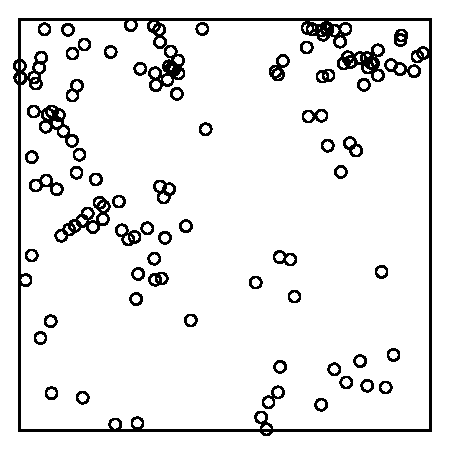
\includegraphics[width=0.4\textwidth]{lansing_blackoak}}
	  \subfloat[Redoak]{\label{fig:redoak}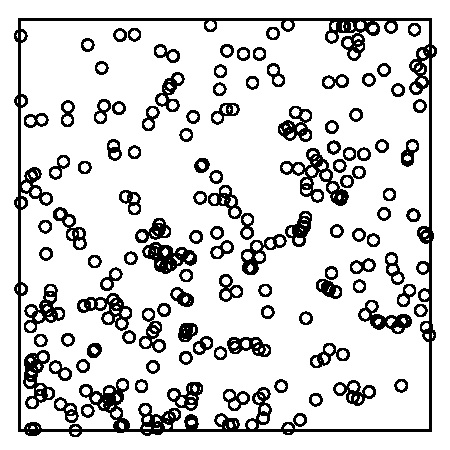
\includegraphics[width=0.4\textwidth]{lansing_redoak}}
	  \subfloat[Whiteoak]{\label{fig:whiteoak}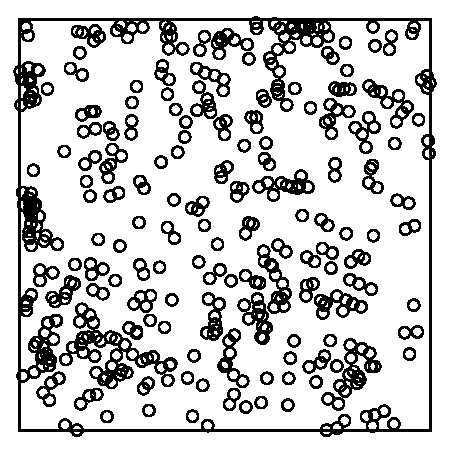
\includegraphics[width=0.4\textwidth]{lansing_whiteoak}}\\
	  \subfloat[Maple]{\label{fig:maple}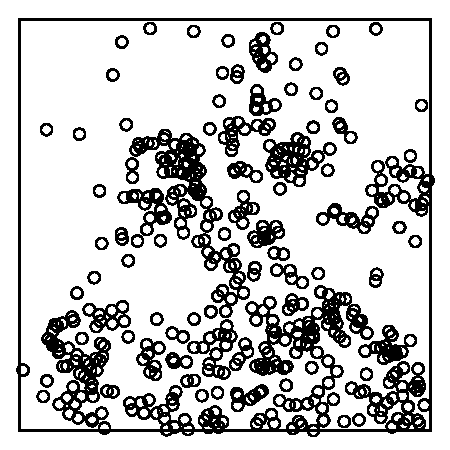
\includegraphics[width=0.4\textwidth]{lansing_maple}}
	  \subfloat[Hickory]{\label{fig:hickory}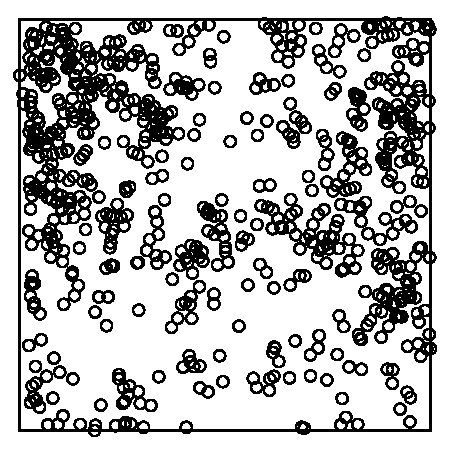
\includegraphics[width=0.4\textwidth]{lansing_hickory}}
	  \subfloat[Misc]{\label{fig:misc}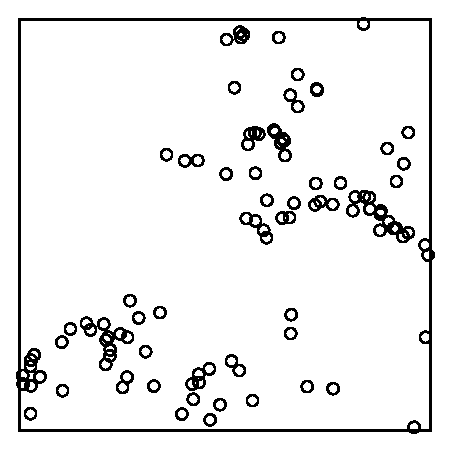
\includegraphics[width=0.4\textwidth]{lansing_misc}}
  \end{adjustwidth}
  \caption{The Lansing Woods dataset}
  \label{fig:lansing_separate}
\end{figure}

 \section{Preprocessing}

The different oaks, namely the black, the white and the redoaks seem to
display rather homogenous intensities judging from the point patterns.
Taking into account the prior information, that these oaks tend associate
with each other, it seems reasonable to combine the different oaks into
a single category. Also since there is no information regarding the constitution
of the ``misc'' category, it is discarded from further analysis. The point patterns
resulting from these preprocessing steps are displayed in figure~\ref{fig:lansing_processed}. 

\begin{figure}[htb]
  \begin{adjustwidth}{-2in}{-2in}
	  \centering
	  \subfloat[Maples]{\label{fig:maple}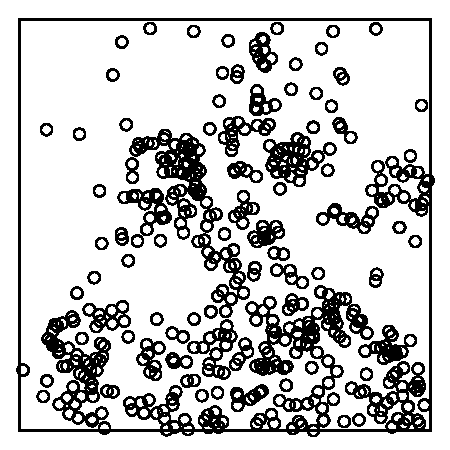
\includegraphics[width=0.4\textwidth]{lansing_maple}}
	  \subfloat[Hickories]{\label{fig:hickory}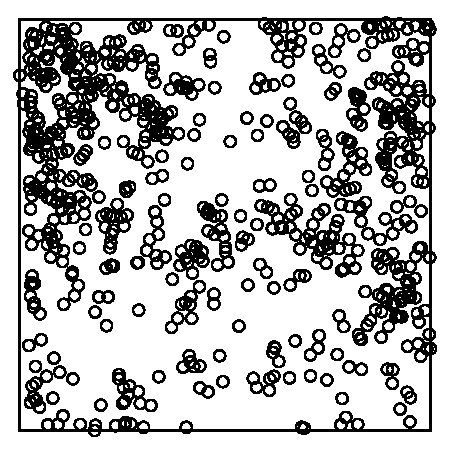
\includegraphics[width=0.4\textwidth]{lansing_hickory}}
	  \subfloat[Oaks]{\label{fig:oak}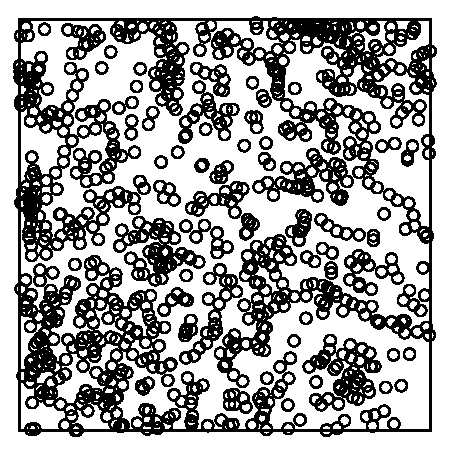
\includegraphics[width=0.4\textwidth]{lansing_oaks_combined}}
  \end{adjustwidth}
  \caption{The dataset after preprocessing}
  \label{fig:lansing_processed}
\end{figure}


\section{Intensity analysis}

It's obvious just by looking at figure~\ref{fig:lansing_separate} that 
the intensity profiles exhibit significant interspecies variability. For example
oaks seems to have almost homogenous intensity whereas maples
displays a much more inhomogenous pattern. A Gaussian kernel smoothed intensity 
estimate is displayed in figure~\ref{fig:intensity_relative}, where
the intensities are comparable between species. 

The most striking conclusion from figure~\ref{fig:intensity_relative} is that
the patterns for hickories and maples are almost complementary. The intensity
of the oaks varies somewhat, but it seems that there are some oaks pretty
much everywhere in the window.

More conclusions can be drawn by plotting some combined point patterns. In 
figure~\ref{fig:combined_intensities} there are all the trees plotted together, then
the oaks and finally the maples and the hickories combined. Indeed, it seems
that when plotted in these combinations, it would be reasonable to assume
constant intensities. We can already come to the following
conclusions
\begin{itemize}
  \item discarding the marks, the intensity of trees is homogenous
  \item oaks are independent of other species
  \item hickories and maples show strong segregation
\end{itemize}

\begin{figure}[htb]
  \begin{adjustwidth}{-2in}{-2in}
	  \centering
	  \subfloat[Maples]{\label{fig:int_maple}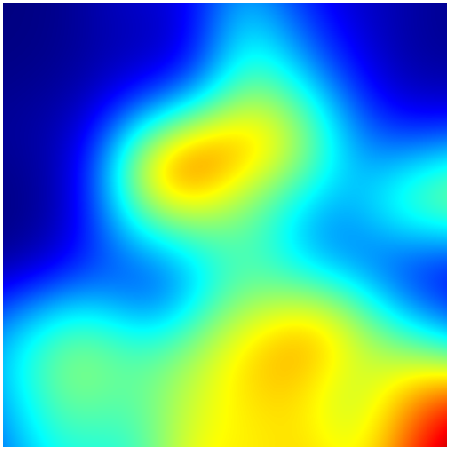
\includegraphics[width=0.4\textwidth]{intensity_relative_maple}}
	  \subfloat[Hickories]{\label{fig:int_hickory}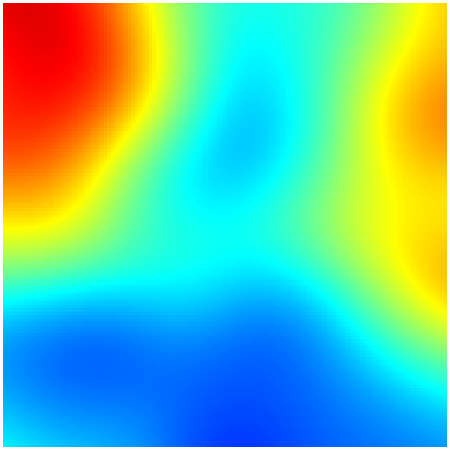
\includegraphics[width=0.4\textwidth]{intensity_relative_hickory}}
	  \subfloat[Oaks]{\label{fig:int_oak}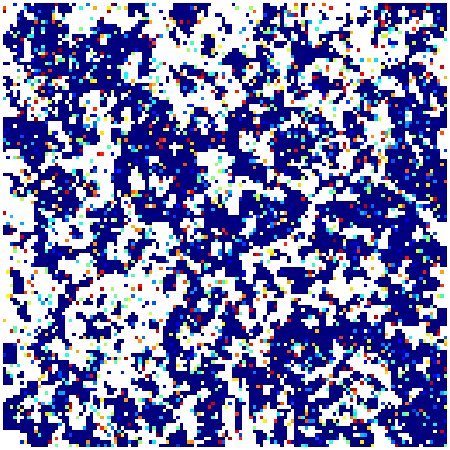
\includegraphics[width=0.4\textwidth]{intensity_relative_oak}}
  \end{adjustwidth}
  \caption{Gaussian Kernel smoothed intensity estimates}
  \label{fig:intensity_relative}
\end{figure}



\begin{figure}[htb]
  \begin{adjustwidth}{-2in}{-2in}
	  \centering
	  \subfloat[All trees]{\label{fig:all_combined}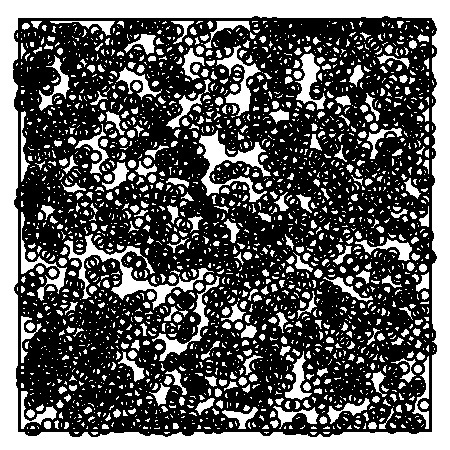
\includegraphics[width=0.4\textwidth]{lansing_all_combined}}
	  \subfloat[Oaks]{\label{fig:oaks_combined}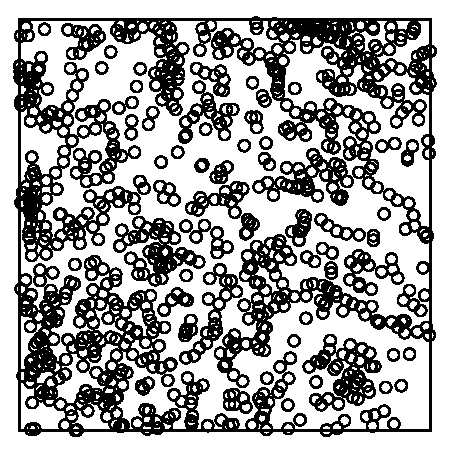
\includegraphics[width=0.4\textwidth]{lansing_oaks_combined}}
	  \subfloat[Hickories \& Maples]{\label{fig:hm_combined}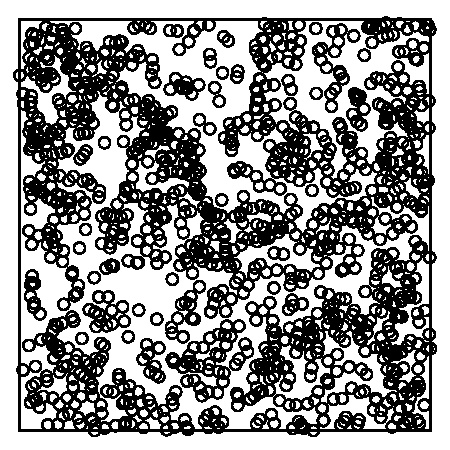
\includegraphics[width=0.4\textwidth]{lansing_hm_combined}}
  \end{adjustwidth}
  \caption{Point patterns with different combinations of the marks in the dataset. The patterns display homogenous intensity.}
  \label{fig:combined_intensities}
\end{figure}

\section{Marking model}



\section{Interaction analysis}

Next we will attempt to characterize the interactions within a single species
and amongst different species.

\subsection{Intra-species interaction}

I have plotted the inhomogenous L-functions \cite{illian}\cite{gelfand} for the maples
and hickories and the ordinary L-function for the oaks.
These are displayed in figure~\ref{fig:intra_interactions}.



\begin{figure}[htb]
  \begin{adjustwidth}{-2in}{-2in}
	  \centering
	  \subfloat[Maples]{\label{fig:l_maple}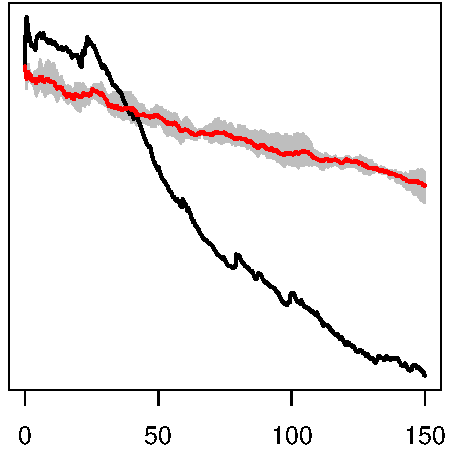
\includegraphics[width=0.4\textwidth]{l_maple}}
	  \subfloat[Hickories]{\label{fig:l_hickory}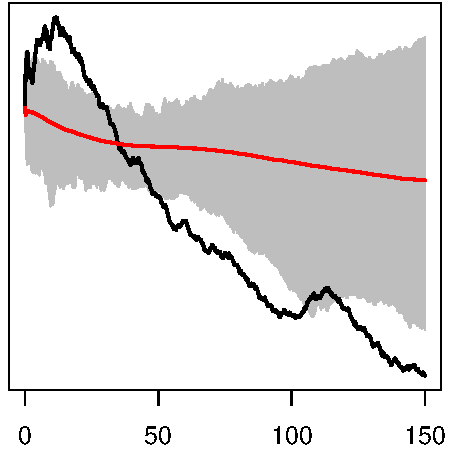
\includegraphics[width=0.4\textwidth]{l_hickory}}
	  \subfloat[Oaks]{\label{fig:l_oak}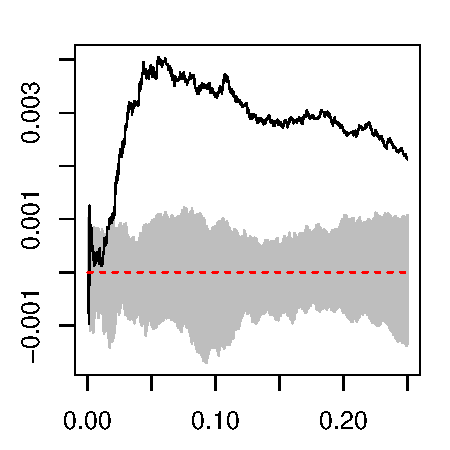
\includegraphics[width=0.4\textwidth]{l_oak}}\\
	  \subfloat[Hickories \& Maples]{\label{fig:l_hm}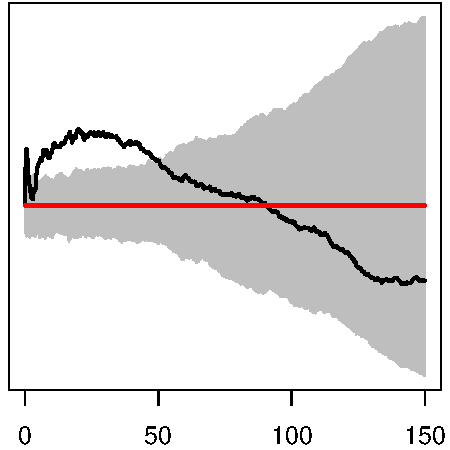
\includegraphics[width=0.4\textwidth]{l_hm}}
	  \subfloat[All trees]{\label{fig:l_all}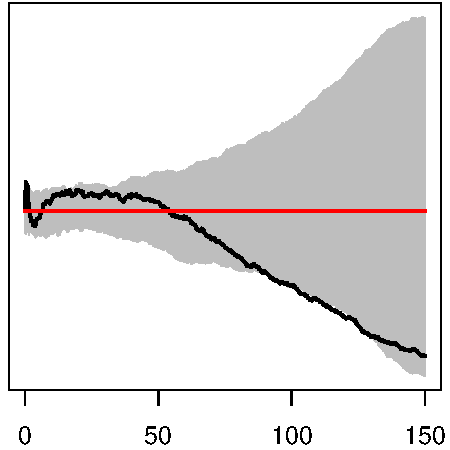
\includegraphics[width=0.4\textwidth]{l_all}}
  \end{adjustwidth}
  \caption{Besag's L-function for the different species. For maples and hickories the inhomogenous version was used. In all of the
  figures there are the envelopes after $20$ monte carlo tests assuming complete spatial randomness.}
  \label{fig:intra_interactions}
\end{figure}


\subsection{Inter-species interaction}

The interspecies interaction was quantified by using the two
different summary statistics: the \emph{partial pair correlation function} (PPCF)
and the \emph{mark connection function}. These can both be interpreted
as displaying the probability, that there is a point of species $i$
an $r$ distance away from a point of species $j$. The plots have been made
for all the pairings $i,j$ from the three species, resulting
in $6$ different plots (pairings of type $i,i$ are also included).
The PPCF is displayed in figure~\ref{fig:pcf} and the mark-connection function
in figure~\ref{fig:markc}. As can be seen, both of them show quite similar
results.


\begin{figure}[htb]
  \begin{adjustwidth}{-2in}{-2in}
	  \centering
	  \subfloat[Mark-connection function]{\label{fig:markc}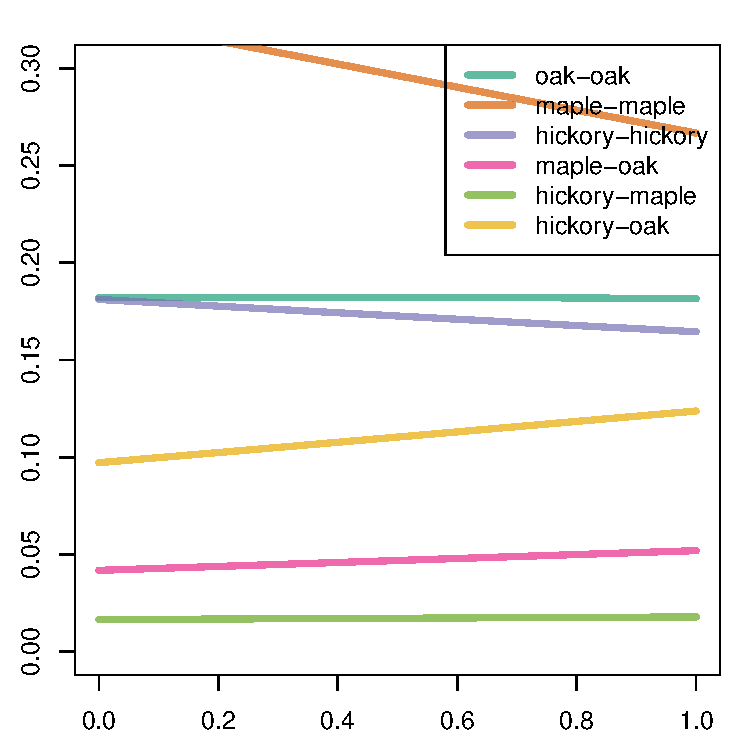
\includegraphics[width=0.7\textwidth]{markc}}
	  \subfloat[PPCF]{\label{fig:pcf}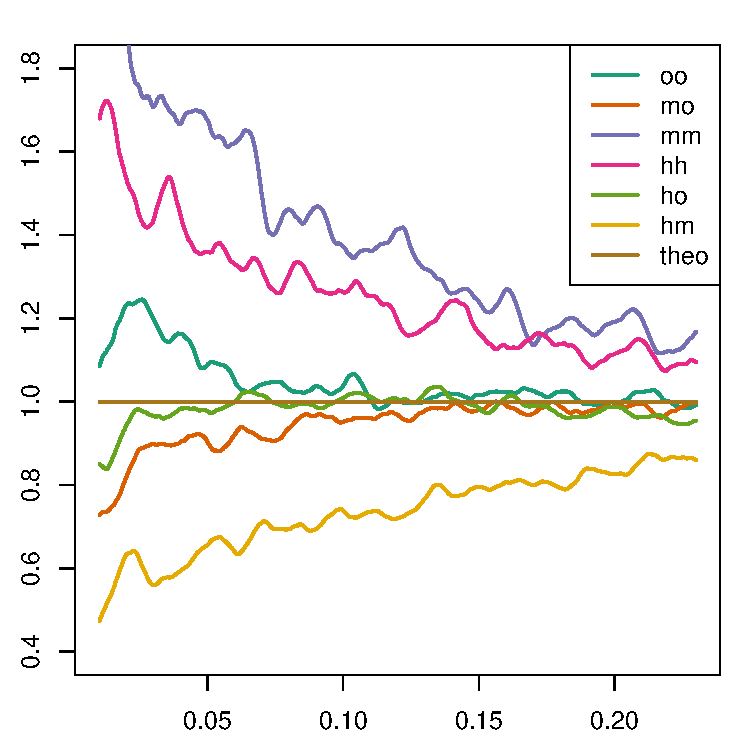
\includegraphics[width=0.7\textwidth]{pcf}}
  \end{adjustwidth}
  \caption{The mark-connection function and the partial pair-correlation function that measure intra- and interspecies interactions.}
\end{figure}

\clearpage

\section{Methods}

\section{Results}

\section{Conclusion}


\printbibliography
\clearpage
\appendix
\section*{R code}

\lstinputlisting{lansing.R}

\end{document}
